\documentclass[a4paper,titlepage,12pt]{article}
\usepackage[utf8]{inputenc} %Make sure all UTF8 characters work in the document
%\usepackage{color}
\usepackage{graphicx}
\usepackage{titling}
\usepackage{tabularx}
\usepackage{longtable}
\usepackage[yyyymmdd]{datetime}
\usepackage[figurename=Figur]{caption}
\usepackage{booktabs}
\usepackage[parfill]{parskip}

%Set page size
\usepackage{geometry}
\geometry{margin=3cm}

\renewcommand{\dateseparator}{-}
\renewcommand{\contentsname}{Innehållsförteckning}

%%%%%%%%%%%%%%%%%%%%%%%%%%%%%%%
% Header and footer
%%%%%%%%%%%%%%%%%%%%%%%%%%%%%%%
\usepackage{fancyhdr}
\pagestyle{fancy}

\lhead{
\includegraphics[width=0.15\linewidth]{../images/logo_full.png}}
\chead{Systemskiss för sexbent robot}
\rhead{\today}
\setlength\headheight{26pt} 

\lfoot{TSEA29 -- KMM \\ LIPS Systemskiss}
\rfoot{Grupp 9 \\ LiTHe Hex}

\newcommand{\itc}{I\textsuperscript{2}C}

\pretitle{%
    \begin{center}
        \LARGE
        
\includegraphics[width=6cm]{../images/logo_full.png}\\[\bigskipamount]
}

\posttitle{\end{center}}

\begin{document}
    \title{\LARGE
        \textbf{Systemskiss för sexbent robot} \\
        \vspace*{0.5\baselineskip}
        \large
        Redaktör Frans Skarman \\
        Grupp 9 \\
        \small
        \vspace*{0.5\baselineskip}
        Version 0.1}

    \date{\today}

	\maketitle
	
	\newpage
	
	\begin{center}

		%%%%%%%%%%%%%%%%%%%%%%%%%%%%%%%%%%%%%%%%%%%%%%%%%%%%%%%%%%%%%%%%%%%%%%%%%%%%%%%%%
		%						Medlemmar
		%%%%%%%%%%%%%%%%%%%%%%%%%%%%%%%%%%%%%%%%%%%%%%%%%%%%%%%%%%%%%%%%%%%%%%%%%%%%%%%%%

		\section*{Projektidentitet}
		Grupp 9, Ht 2016, LiTHe Hex

		Linköpings Tekniska Högskola, ISY

		\renewcommand*{\arraystretch}{1.4}
		\begin{longtable}[c]{ l l l }
			\textbf{Namn} & \textbf{Ansvar} & \textbf{E-post} \\ \midrule
			Emil Segerbäck & & emise935@student.liu.se \\ \midrule
			Frans Skarman & Dokumentansvarig & frask812@student.liu.se \\ \midrule
			Hannes Tuhkala & & hantu447@student.liu.se \\ \midrule
			Malcolm Vigren & Projektledare & malvi108@student.liu.se \\ \midrule
			Noak Ringman &  & noari093@student.liu.se \\ \midrule
			Olav Övrebö &  & olaov121@student.liu.se \\ \midrule
			Robin Sliwa &  & robsl733@student.liu.se \\
		\end{longtable}

		\centering
		\textbf{Kursansvarig}: Tomas Svensson Rum 3B:528 013--28 13 68 tomas.svensson@liu.se

		\newpage
		\tableofcontents
		\newpage


		%%%%%%%%%%%%%%%%%%%%%%%%%%%%%%%%%%%%%%%%%%%%%%%%%%%%%%%%%%%%%%%%%%%%%%%%%%%%%%%%%
		%						Historik
		%%%%%%%%%%%%%%%%%%%%%%%%%%%%%%%%%%%%%%%%%%%%%%%%%%%%%%%%%%%%%%%%%%%%%%%%%%%%%%%%%

		\section*{Dokumenthistorik}
		\renewcommand*{\arraystretch}{1.4}
		\begin{longtable}[c]{ l l l l l }
			\textbf{Version} & \textbf{Datum} & \textbf{Utförda förändringar} 
			& \textbf{Utförda av} & \textbf{Granskad} \\ \midrule
			
			0.1 & 2016--09--20 & Första utkastet & Projektgruppen & \\
		\end{longtable}
	\end{center}

	%%%%%%%%%%%%%%%%%%%%%%%%%%%%%%%%%%%%%%%%%%%%%%%%%%%%%%%%%%%%%%%%%%%%%%%%%%%%%%%%%
	%						Inledning
	%%%%%%%%%%%%%%%%%%%%%%%%%%%%%%%%%%%%%%%%%%%%%%%%%%%%%%%%%%%%%%%%%%%%%%%%%%%%%%%%%

	\newpage

	\section{Inledning}
	I detta dokument beskrivs delsystemen mer ingående samt förslag på hur de ska 
    implementeras. De delsystem som roboten ska använda sig av är:
	Centralenhet, motorikenhet och sensorenhet.

	%%%%%%%%%%%%%%%%%%%%%%%%%%%%%%%%%%%%%%%%%%%%%%%%%%%%%%%%%%%%%%%%%%%%%%%%%%%%%%%%%
	%						Översikt
	%%%%%%%%%%%%%%%%%%%%%%%%%%%%%%%%%%%%%%%%%%%%%%%%%%%%%%%%%%%%%%%%%%%%%%%%%%%%%%%%%

  \newpage
	\section{Systemöversikt}
	Systemet ska innehålla tre enheter. En centralenhet för kommunikation med en
    dator, en motorikenhet som sköter hur benen rör sig samt en sensorenhet som
    tolkar sensordata. Centralenheten är även den enhet som tar beslut och
    kommunicerar med de andra enheterna. Se Figur.~\ref{fig:overview} för en översiktsbild av
    systemet.
	\begin{figure}[h]
		\centering
		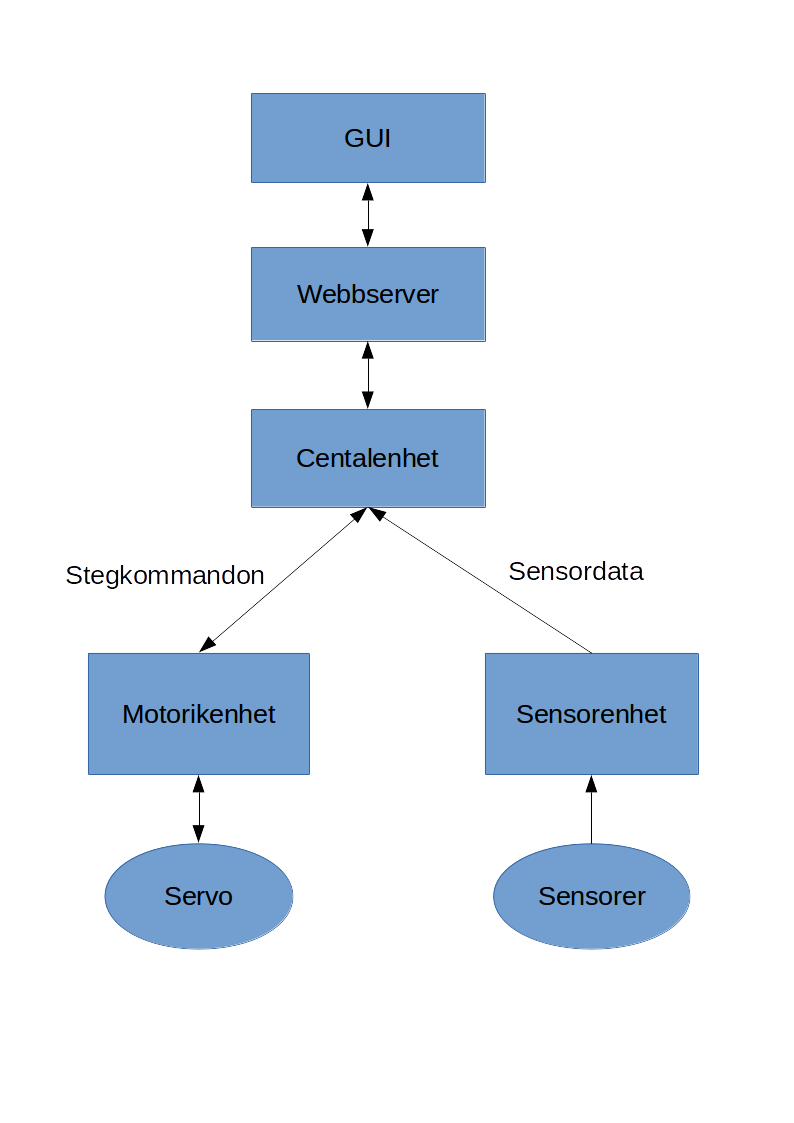
\includegraphics[width=0.5\linewidth]{../images/overview.png}
		\caption{Översikt av systemet\label{fig:overview}}
	\end{figure}

	\subsection{Kommunikation mellan enheterna}
	Kommunikation kan ske med UART, SPI eller \itc{}. AVR-processorerna har
	2 UART-, 3 SPI- och en \itc{}-ingång medan Raspberry PI:en har 1 UART-, 2 SPI- och
	en \itc{}-ingång. 

	\subsubsection{Förslag 1}
	Om vi vill ha en LIDAR-avståndsmätare kommer sensorenhetens \itc{}-port att gå åt
	till kommunikation med avståndsmätaren. Sensorenheten måste alltså kommunicera med
	centralenheten via UART eller SPI.\@ Om kommunikationen sker med UART måste 
	motorikenheten kommunicera med SPI eftersom att centralenheten endast har en
	UART port.

	\subsubsection{Förslag 2}
	Om både motorikenheten och sensorenheten har sin \itc{}-buss tillgänglig kan de
	kommunicera med centralenheten via en gemensam \itc{}-buss där
	centralenheten är master och de andra enheterna är slaves. 
	
	\section{Centralenheten}
	Centralenheten har tre ansvarsområden: navigation/beslutsfattning, hinderdetektion samt
	kommunikation med omvärlden.

	\subsection{Navigation och beslutsfattning}
  
  \subsubsection{Förslag 1}
  Centralenheten frågar om data från sensorenheten varje gång det ska fattas ett
  beslut. Detta gör att centralenheten själv bestämmer när den ska ha ny data
  för att den inte ska bli avbruten eller missa data för att den är mitt i
  utförandet av en annan funktion. Utifrån denna data fattar centralenheten
  beslut om hexapodens färdriktning.
  
  \subsubsection{Förslag 2}
  Sensorenheten sänder kontinuerligt data som tas emot av centralenheten och används löpande 
  för att fatta beslut. 
  
	\subsection{Hinderdetektion}
	För hinderdetektering finns det olika alternativ att använda. Det är möjligt att 
	detektera hinder med hjälp av en avståndsmätare som är vinklad nedåt, en IR-sensor 
	eller LIDAR kan användas som avståndsmätare. Att använda en IR-sensor är fördelaktigt 
	då IR-sensorer antagligen kommer att användas för att undvika väggar. En 
	LIDAR är en ny enhet och medför ett ytterligare, mer avancerat gränssnitt. Ett annat 
	alternativ för att upptäcka hinder är att läsa av det motstånd som benens servo kan 
	returnera tillsammans med övriga sensorer för att upptäcka när roboten går in i ett 
	hinder. 

	\subsection{Kommunikation}
	Centralenheten ska kommunicera med en dator över WiFi. Det är datorns webbläsare 
	som kommer att ansluta till centralenhetens webbserver, det blir då möjligt
    via webbgränssnittet att styra roboten samt läsa av robotens loggar. Det finns
    flera gränssnitt att 
	använda för kommunikation mellan processorerna. Intressanta gränssnitt är SPI, 
	\itc{} och UART.\@ UART är inte möjligt att använda till sensorenheten och 
	motorikenheten då Raspberry Pi endast har en UART port. Både 
	SPI och \itc{} kan användas förutsett att LIDAR inte används. (Endast en 
	\itc{} port finns på sensorenheten, vilken i så fall måste gå till LIDAR,vilken 
	endast använder detta protokoll.) \itc{} måste konfigureras med ett
    master-/slave-förhållande. Centralenheten behöver vara master för att kunna
    kommunicera med 
	sensorenheten och motorikenheten som är slave. Med den konfigurationen blir 
	det inte möjligt för sensorenhet och motorikenheten att kommunicera med
	centralenheten utan att centralenheten har på startat kommunikationen. I och 
	med att \itc{} behöver en master/slave konfiguration blir SPI enklare att använda 
	för tvåvägskommunikation. 



	%%%%%%%%%%%%%%%%%%%%%%%%%%%%%%%%%%%%%%%%%%%%%%%%%%%%%%%%%%%%%%%%%%%%%%%%%%%%%%%%%
	%						Motorikenheten
	%%%%%%%%%%%%%%%%%%%%%%%%%%%%%%%%%%%%%%%%%%%%%%%%%%%%%%%%%%%%%%%%%%%%%%%%%%%%%%%%%
	
	\section{Motorikenheten}
    	Motorikenheten översätter signaler från centralenheten, angeende önskad förflyttning, 
    	till instruktioner för benens förflyttning, och förser centralenheten med data om
    	benens motstånd.
    
    	\subsection{Alternativ 1: Anpassad gångstil}
    	Motorikenheten mottar instruktioner från centralenheten, angeende önskad hastighet, 
    	rotation och riktning för förflyttnnig. Den behandlar detta och räknar ut en lämplig 
	gångstil, och signalerar nödvändiga vinklar till de sex benen. Vissa delmoment i 
	förflyttningen görs hårdkodade. 
    
    	\subsubsection{Planläggning}
	Första steget i motorikenheten för en anpassad gångstil är att utifrån efterfrågad
    	förflyttning avgöra en önskad slutposition för respektive ben, som för roboten närmre 
    	ett läge angivet av centralenheten. Utifrån hastighet kan förflyttningsvektorerna 
    	från nuvarande läge för nuvarande ben skalas ner eller upp, inom rimligheten för vad
    	benen kan nå. För flyttning sker för vänster fram- och bak-ben och höger 
    	mittben, eller för höger fram- och bak-ben och vänster mittben, alternerande för varje
    	förflyttningscykel. När ett sett förflyttas, skiftas de markfästa benen vid behov för 
    	att flytta själva kroppen. Inför ett steg med ett ben hårdkodas ett lyft av benet. 
	Även bestigning av hinder kan komma att hårdkodas.
    
    	\subsubsection{Invers kinematik}
    	Andra steget i motorikenheten för en anpassad gångstil är beräkning av benens vinklar;
    	utifrån kända längder på benen  och önskad vågrät vinkel och längd till slutposition 
    	används trigonometri för att avgöra slutgiltiga aktuatorvinklar.
    
    	\subsection{Alternativ 2: Hårdkodad}
    	Motorikenheten förses med en uppsättning hårdkodade instruktioner för benrörelser, och
    	väljer bland dessa utifrån försedda indata. Hårdkodade rörelser inkluderar rotation på 
    	plats, rörelse framåt (två hastigheter), bakåt och i sidled, rörelse med svag rotation, 
    	bestigning av hinder (i mån av uppfyllande av detta sekundära krav). 
	
	%%%%%%%%%%%%%%%%%%%%%%%%%%%%%%%%%%%%%%%%%%%%%%%%%%%%%%%%%%%%%%%%%%%%%%%%%%%%%%%%%
	%						Sensorenheten
	%%%%%%%%%%%%%%%%%%%%%%%%%%%%%%%%%%%%%%%%%%%%%%%%%%%%%%%%%%%%%%%%%%%%%%%%%%%%%%%%%
	\section{Sensorenheten}
    
    Sensorenheten är den enhet som ger roboten sinnen för omvärlden, så att den
    kan navigera autonomt genom labyrinten. Sensorenheten ska för
    centralenheten vara ett abstrakt gränssnitt till sensorerna. Centralenheten
    behöver alltså inte veta exakt vilka sensorer som används, utan istället
    läser av data som "avstånd till vägg", eller "vridning relativt väggarna".

    \subsection{Gyro}
    
    Sensorenheten ska använda ett gyro för att mäta vridning i det horizontella
    planet. Detta är användbart bland annat för att roboten ska veta hur mycket
    den ska rotera när den svänger.
    
    \subsection{Avståndssensorer fram}
    
    Sensorenheten ska använda avståndssensorer på framsidan, en sensor för att
    upptäcka väggar, och en sensor, snett vinklat ner mot golvet, för hinderdetektion. 

    Avståndssensorn som mäter framåt ska utgöras av en IR-sensor, med
    tillräckling räckvidd för att kunna avgöra om det den tittar på är en
    återvändsgränd eller inte, utan att först behöva gå in i den eventuella
    återvändsgränden.

    \subsubsection{Sensor för hinderdetektion -- förslag 1}

    Sensorn som ska upptäcka hinder ska utgöras av en IR-sensor. Detta
    har fördelen av att ha samma gränssnitt som de andra IR-sensorerna roboten
    ska använda.

    \subsubsection{Sensor för hinderdetektion -- förslag 2}

    Sensorn för hinderdetektion utgörs av en laser-sensor (LIDAR). Denna har
    fördelen av att vara mycket mer exakt än en IR-sensor, men nackdelen av att
    ha ett \itc{}-gränssnitt som ingen annan sensor har, som ökar
    komplexiteten hos sensorenheten.

    \subsection{Avståndssensorer åt sidorna}
    Roboten ska ha avståndssensorer på vardera långsida av roboten, för
    detektion av väggar och återvändsgränder.

    \subsubsection{Väggsensorer -- förslag 1}
    
    En ultraljudssensor på vardera sida. Denna sensortyp har fördelen av att ha
    räckvidden 3 cm till 3 m, vilket borde ge god precision för både upptäckt
    av väggar samt återvändsgränder.

    \subsubsection{Väggsensorer -- förslag 2}

    En IR-sensor på vardera sida. Denna typ har fördelen av att vara mer exakta
    än ultraljudssensorer, men har smalare räckviddsområde.

    \subsubsection{Väggsensorer -- förslag 3}

    Två IR-sensorer används på vardera sida, båda pekande ut från samma sida och
    placerade på vardera ända av plattformen. Detta möjliggör mätning av hur
    roboten är vriden i en rak korridor, och kan användas som fel-kontroll av
    gyrot.

    \subsubsection{Väggsensorer -- förslag 4}

    Samma som förslag 3, fast två av sensorerna är ultraljudssensorer, ifall
    IR-sensorerna stör ut varandra.

    \subsection{Styrenhet}

    Styrenheten för sensorenheten ska bestå av en AVR-processor, som läser av och behandlar
    informationen från robotens sensorer. Styrenheten sköter även
    kommunikationen med centralenheten -- den tar emot förfrågningar om data och
    skickar behandlad data på begäran.

    Styrenheten ska behandla den råa sensordatan till den grad att
    centralenheten inte behöver allt för mycket egna beräkningar på
    sensorinformationen. Den ska därför bland annat sköta brusreducering av
    datan, samt beräkna integralen av informationen från gyrot för att få ut en
    faktisk vinkel som roboten roterat. Om två avståndssensorer på vardera sida
    av roboten ska användas, ska styrenheten även beräkna robotens relativa
    orientering till väggen.
    

	%%%%%%%%%%%%%%%%%%%%%%%%%%%%%%%%%%%%%%%%%%%%%%%%%%%%%%%%%%%%%%%%%%%%%%%%%%%%%%%%%
	%						Grafiskt användargränssnitt
	%%%%%%%%%%%%%%%%%%%%%%%%%%%%%%%%%%%%%%%%%%%%%%%%%%%%%%%%%%%%%%%%%%%%%%%%%%%%%%%%%
	\section{Grafiskt användargränssnitt}
    
    På centralenheten ska en webbserver köras som tillhandahåller ett gränssnitt
    för användaren där man kan läsa sensordata eller kontrollera roboten i
    manuellt läge. Front-end ska skrivas i Elm och back-end i Elixir.

    I det manuella läget styras med en joystick som är kopplad till användarens
    dator.
    
    Eventuellt ska även video från en kamera på roboten streamas till gränssnittet.
    

	%%%%%%%%%%%%%%%%%%%%%%%%%%%%%%%%%%%%%%%%%%%%%%%%%%%%%%%%%%%%%%%%%%%%%%%%%%%%%%%%%
	%						Simuleringar
	%%%%%%%%%%%%%%%%%%%%%%%%%%%%%%%%%%%%%%%%%%%%%%%%%%%%%%%%%%%%%%%%%%%%%%%%%%%%%%%%%
	\section{Simuleringar}
    För att underlätta utvecklingen av vissa delar av projektet kommer vi att skriva
	kod för att simulera de delarna. Simuleringarna ska kunna köra samma kod som ska
	köras på roboten men visualisera resultatet utan resten av roboten. De två
	delarna där simulering är mest aktuellt är inverse kinematics och gångstilskoden.

\end{document}
